\section{File System Security}
% ----------
\subsection{Files permissions}
A chaque utilisateur est assigné un user ID (UID). Chaque utilisateur peut être membre d'un ou plusieurs groupes (désigné par des groupes ID - GID).

La list des utilisateurs peut être consultées dans le fichier \verb+/etc/passwd+.

La liste des groupes est disponible sur le fichier \verb+/etc/group+.

Les mots de passes se trouvent dans le fichier \verb+/etc/shadow+.
\begin{figure}[H]
    \centering
    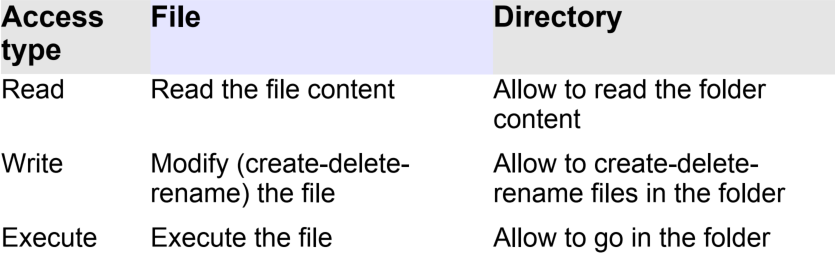
\includegraphics[width=0.8\columnwidth]{fileperm.png}
\end{figure}
% ----------
\subsection{Real-effective userID and groupID}
Chaque processus possède un effective UID et un real UID, idem pour les GID.

Linux utilise seulement le effective userID. Si le bit userID est actif alors le fichier exécuté prend les droits du propriétaire du fichier.

\subsection{ACL - Access Control List}
Les filesystems ext3,ext4,tmpfs,btrfs autorise les ACL
u: : User, g: : Group, o: : Other
\begin{lstlisting}[style=bash]
setfacl -m u::rwx,g::r--,o:--- test
setfacl -Rm u:user1:rw TestDirectory # -R: Recursive
# remove
setfacl -b test #The file test has no ACL
setfacl -x u:user1,g:group1 test #The file test has no rights for user1
and group1
\end{lstlisting}

\subsection{Attributs particuliers des FS ext2-3-4}
On peut utiliser la commande \verb!lsattr! ou \verb!chattr!
\begin{lstlisting}[style=bash,label={lst:attribus},caption={}]
chattr +i file #add i attribute
chattr -i file #del i attribute
chattr =i file #equal i attribute
lsattr file
\end{lstlisting}
\begin{itemize}
\item -i :file/directory can not be modified, deleted, renamed or linked symbolically, not even by root. Only root or a binary with the necessary rights can set this attribute.
\item -A :Date of last access is not updated (only useful for reducing disk
access)
\item -S :File is synchronous, the records in the file are made immediately on the disc. (equivalent to the sync option of mount)
\item -a :File can only be open in append mode for writing (log files, etc.) Only redirection $>>$ can be used, the file can not be deleted.
\item -c :File is automatically compressed before writing to disk, and unpacked before playback
\item -d :File will not be saved by the dump
\item -j :Ext3-ext4 :A file with the 'j' attribute has all of its data written to
the ext3 or ext4 journal before being written to the file itself
\item -s :When the file is destroyed, all data blocks are being released to zero.
\end{itemize}

\subsection{Recherche de permissions faibles}
\begin{lstlisting}[style=bash,label={lst:perm},caption={}]
find . -perm 200 #file permissions = 200
find . -perm -220 #write bit for user and group = 1
find . -perm /220 #write bit for user or group = 1
find . -perm +220 #write bit for user or group = 1 (like /220)
\end{lstlisting}

\subsection{Sécuriser les répertoires temporaires}
\begin{itemize}
\item mettre le \verb!\tmp! dans une autre partition
\item no suid programme sont permis
\item rien ne peut être exécuté 
\item aucun node file existe dans le \verb!\tmp!
\end{itemize}

\subsection{Mémorisation des mots de passes}
Les mot de passes sont sotckés en HASH (preuve sans connaissance) dans le fichier \verb+/etc/shadow+.